\documentclass{article}

\usepackage{graphicx} % Required for inserting images
\usepackage{geometry}
\usepackage{float}
\usepackage{tabularray}
\usepackage{listings}


\begin{document}

\begin{titlepage}
    \centering
    \vspace*{1cm}

    
\includegraphics[width=0.4\textwidth]{Images/dei_thumb.png} % Replace with your university logo

    \vspace{1.5cm}
    {\LARGE \textbf{Teste Dinâmico de Software} \par}
   
    

    \vspace{2.5cm}
    \textbf{Mestrado em Engenharia Informática} \\
    \textbf{Qualidade e Confiabilidade de Software 2023/2024} \\
    \vspace{0.5cm} 
    \textbf{Versão do Documento: 1.0} \\
    \vspace{3cm}
    \begin{tabular}{ll}
        \textbf{Bruno Sequeira} & 2020235721, brunosequeira@student.dei.uc.pt \\
        \textbf{Rui Santos} & 2020225542, rpsantos@student.dei.uc.pt
        
      

    \end{tabular}\\
    \vspace{1.5cm} 
    \textbf{Universidade de Coimbra}

    \date{}

    \vfill

\end{titlepage}
   

\clearpage


\section{Introdução}
\quad Este projeto consiste no desenvolvimento de um plano de teste de software de modo a testar, avaliar e testar um software implementado por outros desenvolvedores.\\ 

\quad O principal objetivo é identificar e selecionar corretamente abordagens de testes dinâmicoss, tendo em conta testes de White Box (que irá ser o mais abordado) e o Black Box, e o que estes dois conceitos podem concluir ao executar um plano de teste de software.

\quad Tal como referido acima, escolhemos dois produtos de software, que são os seguintes:

\begin{itemize}
    \item \textbf{Jogo do Sudoku}: Este código iré tentar resolver uma tela 9x9 com as regras do sudoku, sendo que a função que irá abordar essa implementação é a \textbf{Solve()}, está irá percorrer posição a posição, usando um algoritmo de back-tracking para no final retornar um boleano com o resultado, sendo que se for true então foi possível a sua realização, sendo possível visualizar o seu resultado. O input é um array bi-dimensional, e o output é a solução deste array.
    \item \textbf{Algoritmo de Dijkstra}: Este software consiste em encontrar os caminhos mais curtos entre vértices consoante as ligações entre eles. O input é a criação de um grafo e escolhendo um vértice como origem. O resultado final é um array com as distâncias entre o ponto de origem com todos os outros vértices.

\end{itemize}
Na secção 2 serão apresentados os aspetos de risco de software a ser testado e potenciais riscos. Na secção 3 serão apresentados os elementos e funcionalidades a serem testados e na secção 4 serão descritos os elementos e funcionalidades que não serão testados, assumindo que estes pontos esão corretos e bem implementados. \\
Na secção 5 será apresentado os planos de testes, na secção 6 serão definidos os critérios de realização do plano de testes. Na secção 7 serão identificados todos os elementos que foram entregues como parte e consequência do plano de testes. Na secção 8 apresentaremos as necessidades específicas para execução dos testes. Na secção 9 a distribuição do trabalho por elemento. E por fim, a secção 10, será apresentado as conclusões para os resultados dos testes, descrevendo os defeitos identificados.

\section{Aspetos de risco do software}
Neste trabalho, a seleção criteriosa e a qualidade dos casos de teste assumem um papel crucial, visto que o código em questão foi desenvolvido para fins académicos e pessoais, sem documentação oficial além do código-fonte fornecido. Essa falta de documentação pode dificultar a compreensão inicial do fluxo do programa.

Além disso, a possibilidade de bus no código levanta a necessidade de testes mais rigorosos para garantir a validade dos resultados.

Por outro lado, visto que é apenas um ficheiro Java, a simplicidade do software elimina a preocupação com dependências externas que possam afetar o seu funcionamento.

\section{Elementos e funcionalidades a serem testadas}

Para o software encontrado, iremo-nos focar na função \textbf{Solve} e \textbf{Dijkstra}, sendo que estas irão ser analisadas e serão realizados testes do tipo White Box separadamente em cada função, iremos abordar o control flow e o data flow.



\section{Elementos e funcionalidades a não serem testadas}

\section{Abordagem dos testes}
\subsection{Testes White Box}
Nesta secção estão presentes os testes de White Box para as funções \textbf{Dijkstra()}, do projeto \textit{Algoritmo de Dijkstra}, e  \textbf{Solve()} do projeto \textit{Sudoku}.

Esta abordagem faz a testagem por partes, ou seja, aos detalhes na implementação do código em análise e foca-se nos testes de \textit{Control-Flow}, onde foram analisados todos os caminhos independentes e implementados casos de testes para cada um.

\subsubsection{Control Flow}

Para realização deste método, iremos apresentar passo a passo, a implementação deste. Projetando o grafo de Control Flow de cada função, determinamos a complexidade ciclomática, analisamos os caminho independentes possíveis e verificamos quais deles são possíveis de serem executados. Com isso, iremos determinar casos de teste para cada um dos caminhos encontrados.
\clearpage
\begin{itemize}
    \item \textbf{Função Dijkstra()}
    
       
    \begin{enumerate}
        
        \item \textbf{Grafo de Control Flow}
    \begin{figure}[H]
    \centering
    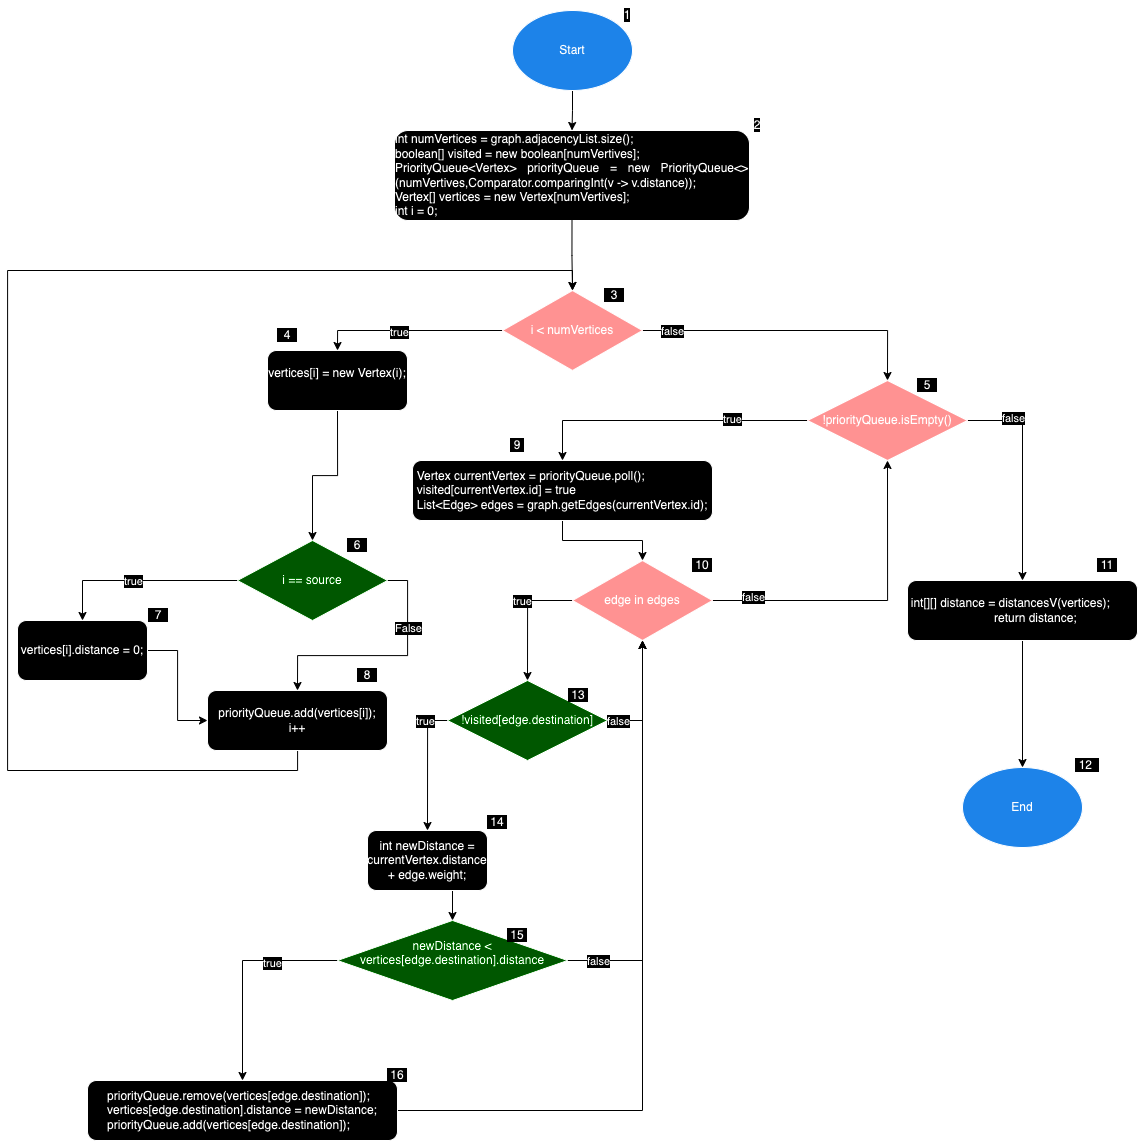
\includegraphics[width=\textwidth]{Images/ControlFlowGraphDijkstra.png}
    \caption{Control Flow - função Dijkstra.} 
    \label{fig:ControlFlow-Dijkstra}

  \end{figure}


  \item \textbf{Complexidade Ciclomática V(G)}
  \quad A complexidade ciclomática é utilizada para determinar o número máximo de caminhos independentes do programa.\\
  \quad A fórmula usada é: \textbf{V(G) = P + 1}.\\

  O \textbf{P} corresponde a nós predicativos.\\

  Nós predicativos são os que têm vários arcos de saída, ou seja, corresponde a condições do programa, tais como, if's, while's e for's.

  \quad Logo, ao analisar a figura de cima, podemos verificar que existem 6 nós predicativos, send o  3  de l es if's (cor verde)  e  3  de l es while's ou for's (cor rosa).

  Portanto a complexidade ciclomática é de 6 + 1 = 7. O que implica que existem no máximo 7 caminhos independentes.
  
  \item \textbf{Caminhos linearmente independentes}\\

  \quad Um caminho linearmente independente é uma sequência de estados de um programa que não pode ser formada combinando outras sequências de estados já testadas, ou seja, é uma sequência única de instruções que representa uma linha de execução distinta no programa.
  Testar caminhos linearmente independentes é importante para garantir uma cobertura abrangente do código.

  Os próximos pontos são os 7 caminhos independentes que encontramos para o código Dijkstra.
  \begin{itemize}
    \item \textbf{P1} = {Start,  2, 3, 5, 11, End}
    \item \textbf{P2} = {Start, 2, 3, 4, 6, 8, 3, 5, 11, End}
    \item \textbf{P3} = {Start, 2, 3, 4, 6, 8, 3, 5, 9, 10, 5, 11, End}
    \item \textbf{P4} = {Start, 2, 3, 4, 6, 7, 8, 3, 5, 9, 10, 5, 11, End}
    \item \textbf{P5} = {Start, 2, 3, 4, 6, 7, 8, 3, 5, 9, 10, 13, 10, 5, 11, End}
    \item \textbf{P6} = {Start, 2, 3, 4, 6, 7, 8, 3, 5, 9, 10, 13, 14, 15, 10, 5, 11, End}
    \item \textbf{P7} = {Start, 2, 3, 4, 6, 7, 8, 3, 5, 9, 10, 13, 14, 15, 16, 10, 5, 11, End}
  \end{itemize}
  NOTA: Start e End correspondem aos estados 1 e 12, respetivamente.

  Destes 7 caminhos linearmente independentes, 2 deles não são executáveis, estes 2 são \textbf{P1} e \textbf{P2}.\\

  \quad Apresentamos agora as razões pelas quais estes não são executáveis são as seguintes: \\
  \begin{itemize}
    \item \textbf{P1} = Neste caso, seria necessário que o grafo não contivesse nenhum elemento, mas para que a funcionalidade da função resulte seria necessário um vértice source, logo o grafo teria de ter pelo menos 1 elemento, só que este iria passar do estado 3 para o estado 4, o que não é o que este caminho deseja. Não sendo possível ser executado.\\
    \item \textbf{P2} = Neste caminho, se o grafo tem de ter pelo menos um elemento, então a fila de vértices é sempre pelo menos um elemento, portanto é impossível a condição do estado 5 ser falsa, visto que no estado 8 é adicionado o elemento na fila. 
  \end{itemize}


  \item \textbf{Casos de teste}\\
 \quad Para cada caminho executável iremos apresentar os casos de usos, com o input e o output desejado.
 O input são várias variáveis, o \textit{numVertices} corresponde ao número de vértices que estão presentes no grafo, o \textit{graph} é o grafo que foi criado com o número de vértices anteriormente apresentada. E o \textit{distance} é o que vai conter o output da função chamada que tem como parâmetros o grafo e o vértice de origem para calcular as distâncias.\\

 O output é um array bi-dimensional que contém as distâncias entre o vértice origem com todos o outros vértices que estão presentes no grafo anteriormente criado.\\


\begin{table}[H]
    \centering
    \begin{tabular}{|c|p{7cm}|p{3cm}|} % Ajusta a largura da coluna "Input" para 5cm
    \hline
    \textbf{Caminho} & \textbf{Input} & \textbf{Output Esperado} \\
                        
    \hline
    \textbf{P3} & int numVertices = 1; \newline
                Graph graph = new Graph(numVertices); \newline
                int[][] distance = dijkstra(graph, 1); & 0 - 2147483647  \\
    \hline
    \textbf{P4} & int numVertices = 1;\newline
    Graph graph = new Graph(numVertices);\newline
    int[][] distance = dijkstra(graph, 0); & 0 - 0 \\
    \hline
    \textbf{P5} & int numVertices = 5;\newline
    Graph graph = new Graph(numVertices);\newline
    graph.addEdge(1,2,1);\newline
    graph.addEdge(2,4,5);\newline
    graph.addEdge(2,3,10);\newline
    graph.addEdge(3,4,3);\newline
    int[][] distance = dijkstra(graph, 0); & 0 - 0\newline
    1 - 2147483647\newline
    2 - 2147483647\newline
    3 - 2147483647\newline
    4 - 2147483647   \\
    \hline
    \textbf{P6} & int numVertices = 2;\newline
    Graph graph = new Graph(numVertices);\newline
    graph.addEdge(0, 1, Integer.MAX\_VALUE); \newline
    int[][] distance = dijkstra(graph, 0); & 0 - 0\newline
    1 - 2147483647 \\
    \hline
    \textbf{P6} & int numVertices = 5;\newline
    Graph graph = new Graph(numVertices);\newline
    graph.addEdge(0,2,1);\newline
    graph.addEdge(0,1,10);\newline
    graph.addEdge(2,4,5);\newline
    graph.addEdge(2,3,10);\newline
    graph.addEdge(3,4,3);\newline
    int[][] distance = dijkstra(graph, 0); & 0 - 0\newline
    1 - 10\newline
    2 - 1\newline
    3 - 11\newline
    4 - 6 \\
    \hline
   
    \end{tabular}
    \caption{Casos de teste para os caminhos independentes do Dijkstra.}
    \label{tab:tabela_exemplo}
\end{table}
\clearpage

  
  

\end{enumerate}
\item \textbf{Sudoku}
\begin{enumerate}
    \item \textbf{Grafo de Control Flow}\\
    \begin{figure}[H]
        \centering
        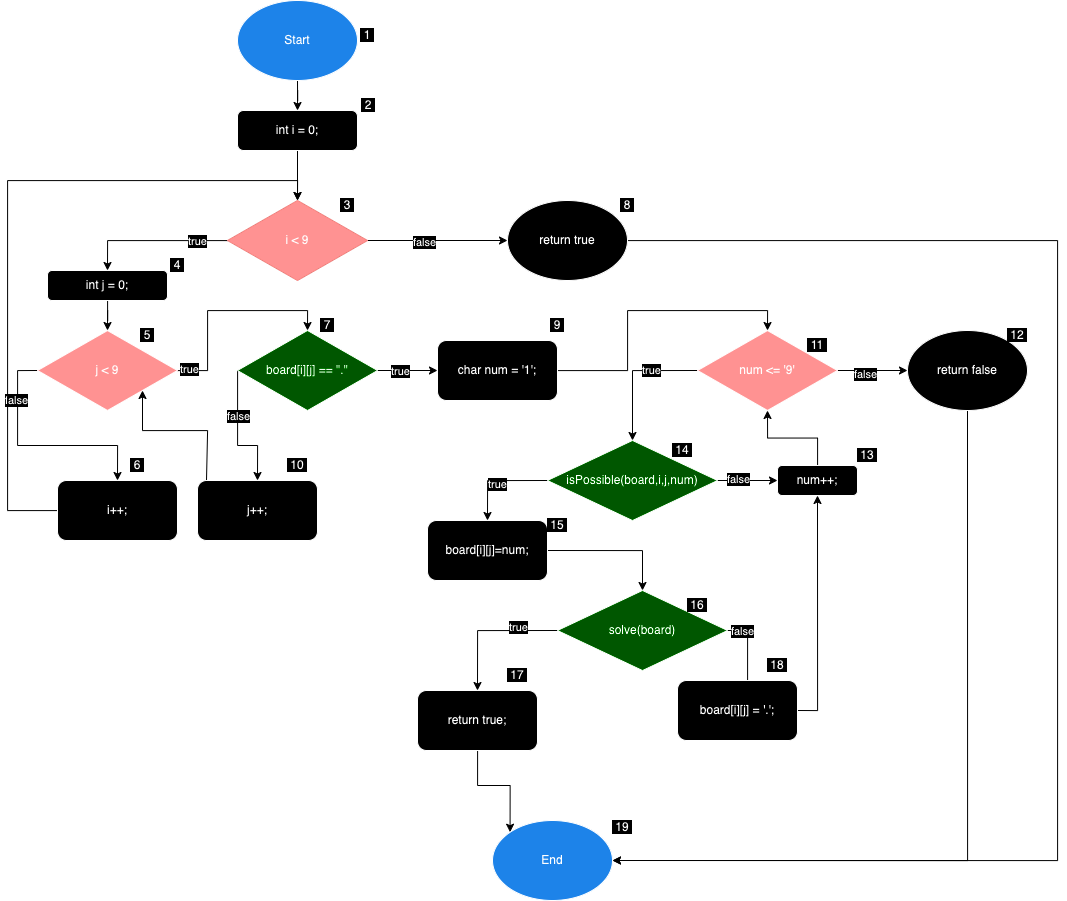
\includegraphics[width=\textwidth]{Images/ControlFlowSudoku.png}
        \caption{Control Flow - função Solve.} 
        \label{fig:ControlFlow-Sudoku}
    \end{figure}
    \item \textbf{Complexidade Ciclomática V(G)}\\
    
    \quad A complexidade ciclomática é utilizada para determinar o número máximo de caminhos independentes do programa.\\
    \quad A fórmula usada é: \textbf{V(G) = P + 1}.\\
  
    O \textbf{P} corresponde a nós predicativos.\\
  
    Nós predicativos são os que têm vários arcos de saída, ou seja, corresponde a condições do programa, tais como, if's, while's e for's.
  
    \quad Logo, ao analisar a figura de cima, podemos verificar que existem 6 nós predicativos, send o  3  de l es if's (cor verde)  e  3  de l es while's ou for's (cor rosa).
  
    Portanto a complexidade ciclomática é de 6 + 1 = 7. O que implica que existem no máximo 7 caminhos independentes.
    
    \item \textbf{Caminhos linearmente independentes}
    Testar caminhos linearmente independentes é importante para garantir uma cobertura abrangente do código.

  Os próximos pontos são os 6 caminhos independentes que encontramos para o código Solve do código Sudoku.
  \begin{itemize}
    \item \textbf{P1} = {Start, 2, 3, 5, 8, End}
    \item \textbf{P2} = {Start, 2, 3, 4, 5, 7, 10, 5, 6, 3, 8, End}
    \item \textbf{P3} = {Start, 2, 3, 4, 5, 7, 9, 11, 14, 15, 16, 17, End} 
    \item \textbf{P4} = {Start, 2, 3, 4, 5, 7, 9, 11, 14, 13, 11, 12, End}
    \item \textbf{P5} = {Start, 2, 3, 4, 5, 7, 9, 11, 14, 13, 11, 14, 15, 16, 18, 13, 11, 14, 13, 11, 12, End}
   \item \textbf{P6} = {Start, 2, 3, 4, 5, 7, 10, 5, 6, 3, 4, 5, 7, 10, 5, 7, 9, 11, 14, 13, 11, 14, 15, 16, 17, End}
    \end{itemize}
    
  Destes 6 caminhos linearmente independentes, 1 deles não é executáveis, o \textbf{P1}.

  \quad Apresentamos agora as razões pelas quais estes não são executáveis são as seguintes: \\
  \begin{itemize}
    \item \textbf{P1} = Neste caso, não encontramos nenhum caso de teste para realização deste caminho, visto que a variável \textbf{i} é inicializada por 0, e a condição seguinte é sempre verdadeira, o que torna assim um caminho \textbf{unfeasable}.

  \end{itemize}
    \item \textbf{Casos de teste}\\
    \quad Para cada caminho executável iremos apresentar os casos de usos, com o input e o output
desejado.
\quad Apresentamos o número do caminho linearmente independente, com o input neste caso o input é o conteúdo da variável \textbf{board} do código que foi submetido do Sudoku, o output é o resultado esperado. Sendo que sempre que existe uma solução este algoritmo altera o board, mas se não encontrar nenhuma solução este irá apresentar o mesmo board que foi submetido.
\begin{table}[H]
    \centering
    \begin{tabular}{|c|p{7cm}|p{3cm}|} % Ajusta a largura da coluna "Input" para 5cm
    \hline
    \renewcommand{\arraystretch}{1.8}
    \textbf{Caminho} & \textbf{Input - Este input é correspondente à variável board.} & \textbf{Output Esperado} \\
                        
    \hline
    \textbf{P2} &   
        {'5', '3', '4', '6', '7', '8', '9', '1', '2'},\newline
        {'6', '7', '2', '1', '9', '5', '3', '4', '8'},\newline
        {'1', '9', '8', '3', '4', '2', '5', '6', '7'},\newline
        {'8', '5', '9', '7', '6', '1', '4', '2', '3'},\newline
        {'4', '2', '6', '8', '5', '3', '7', '9', '1'},\newline
        {'7', '1', '3', '9', '2', '4', '8', '5', '6'},\newline
        {'9', '6', '1', '5', '3', '7', '2', '8', '4'},\newline
        {'2', '8', '7', '4', '1', '9', '6', '3', '5'},\newline
        {'3', '4', '5', '2', '8', '6', '1', '7', '9'}; & 
    5 3 4 6 7 8 9 1 2 \newline
    6 7 2 1 9 5 3 4 8 \newline
    1 9 8 3 4 2 5 6 7 \newline
    8 5 9 7 6 1 4 2 3 \newline
    4 2 6 8 5 3 7 9 1 \newline
    7 1 3 9 2 4 8 5 6 \newline
    9 6 1 5 3 7 2 8 4 \newline
    2 8 7 4 1 9 6 3 5 \newline
    3 4 5 2 8 6 1 7 9   \\
    \hline
    \textbf{P3} & 
        {'.', '.', '.', '.', '.', '.', '.', '.', '.'},\newline
        {'.', '.', '.', '.', '.', '.', '.', '.', '.'},\newline
        {'.', '.', '.', '.', '.', '.', '.', '.', '.'},\newline
        {'.', '.', '.', '.', '.', '.', '.', '.', '.'},\newline
        {'.', '.', '.', '.', '.', '.', '.', '.', '.'},\newline
        {'.', '.', '.', '.', '.', '.', '.', '.', '.'},\newline
        {'.', '.', '.', '.', '.', '.', '.', '.', '.'},\newline
        {'.', '.', '.', '.', '.', '.', '.', '.', '.'},\newline
        {'.', '.', '.', '.', '.', '.', '.', '.', '.'}; & 1 2 3 4 5 6 7 8 9\newline
    4 5 6 7 8 9 1 2 3\newline
    7 8 9 1 2 3 4 5 6\newline
    2 1 4 3 6 5 8 9 7\newline
    3 6 5 8 9 7 2 1 4 \newline
    8 9 7 2 1 4 3 6 5\newline
    5 3 1 6 4 2 9 7 8\newline
    6 4 2 9 7 8 5 3 1\newline
    9 7 8 5 3 1 6 4 2 \\
    \hline
    \textbf{P4} &  
        {'.', '3', '4', '5', '7', '8', '9', '1', '2'},\newline
        {'6', '7', '2', '1', '9', '5', '3', '4', '8'},\newline
        {'1', '9', '8', '3', '4', '2', '5', '6', '7'},\newline
        {'8', '5', '9', '7', '6', '1', '4', '2', '3'},\newline
        {'4', '2', '6', '8', '5', '3', '7', '9', '1'},\newline
        {'7', '1', '3', '9', '2', '4', '8', '5', '6'},\newline
        {'9', '6', '1', '5', '3', '7', '2', '8', '4'},\newline
        {'2', '8', '7', '4', '1', '9', '6', '3', '5'},\newline
        {'3', '4', '5', '2', '8', '6', '1', '7', '9'}; & 
        . 3 4 5 7 8 9 1 2 \newline
        6 7 2 1 9 5 3 4 8 \newline
        1 9 8 3 4 2 5 6 7 \newline
        8 5 9 7 6 1 4 2 3 \newline
        4 2 6 8 5 3 7 9 1 \newline
        7 1 3 9 2 4 8 5 6 \newline
        9 6 1 5 3 7 2 8 4 \newline
        2 8 7 4 1 9 6 3 5 \newline
        3 4 5 2 8 6 1 7 9   \\
\hline
   
    \textbf{P5} & 
        {'.', '.', '4', '6', '7', '8', '9', '1', '2'},\newline
        {'.', '7', '2', '1', '9', '5', '3', '4', '8'},\newline
        {'1', '9', '8', '3', '4', '.', '5', '6', '7'},\newline
        {'8', '5', '.', '7', '6', '1', '4', '2', '3'},\newline
        {'2', '2', '6', '8', '5', '3', '.', '.', '1'},\newline
        {'7', '1', '3', '9', '2', '4', '8', '5', '6'},\newline
        {'9', '.', '1', '.', '3', '.', '2', '8', '4'},\newline
        {'.', '8', '7', '4', '1', '9', '6', '3', '5'},\newline
        {'3', '4', '5', '2', '.', '6', '1', '7', '9'}; & . . 4 6 7 8 9 1 2 \newline
    . 7 2 1 9 5 3 4 8 \newline
    1 9 8 3 4 . 5 6 7 \newline
    8 5 . 7 6 1 4 2 3 \newline
    2 2 6 8 5 3 . . 1 \newline
    7 1 3 9 2 4 8 5 6 \newline
    9 . 1 . 3 . 2 8 4 \newline
    . 8 7 4 1 9 6 3 5 \newline
    3 4 5 2 . 6 1 7 9 \\
    \hline
    \textbf{P6} & 
        {'5', '3', '4', '6', '7', '8', '9', '1', '2'},\newline
        {'6', '7', '2', '1', '9', '5', '3', '4', '8'},\newline
        {'1', '9', '8', '3', '4', '2', '5', '6', '7'},\newline
        {'8', '5', '9', '7', '6', '1', '4', '2', '3'},\newline
        {'4', '2', '6', '8', '5', '3', '7', '9', '1'},\newline
        {'7', '1', '3', '9', '2', '4', '8', '5', '6'},\newline
        {'9', '6', '1', '5', '3', '7', '2', '8', '4'},\newline
        {'2', '8', '7', '4', '1', '9', '6', '3', '5'},\newline
        {'3', '4', '5', '2', '8', '6', '1', '7', '.'}; &5 3 4 6 7 8 9 1 2 \newline
    6 7 2 1 9 5 3 4 8\newline
    1 9 8 3 4 2 5 6 7\newline
    8 5 9 7 6 1 4 2 3\newline
    4 2 6 8 5 3 7 9 1\newline
    7 1 3 9 2 4 8 5 6\newline
    9 6 1 5 3 7 2 8 4\newline
    2 8 7 4 1 9 6 3 5\newline
    3 4 5 2 8 6 1 7 9\\
    \hline
   
    \end{tabular}
    \caption{Casos de teste para os caminhos independentes do Dijkstra.}
    \label{tab:tabela_exemplo}
\end{table}

\end{enumerate}

\end{itemize}
\subsubsection{Data Flow}

O teste de Data flow é uma técnica de teste de white box que examina o fluxo de dados em relação às variáveis usadas no código.\\
É o processo de coleta de informações sobre como as variáveis fluem os dados no programa. Ele tenta obter informações específicas de cada ponto específico no processo. O teste de fluo de dados tem um grupo de estratégias de teste para examinar o fluxo de controlo de programas, a fim de explorar a sequência de variáveis de acordo com a sequência de eventos. Ele se concentra principalmente nos pontos em que os valores são atribuídos às váriaves e o ponto em que estes são usados.\\
\textbf{Vantagem:}\\
O teste de fluxo de dados é usado para encontrar os seguintes problemas:\\
\begin{itemize}
    \item Encontrar uma variável usada, mas nunca definida.
    \item Encontrar uma variável definida, mas nunca usada.
    \item Encontrar uma variável definida várias vezes antes de ser usada.
\end{itemize}

\textbf{Desvantagem:}
O processo é demorado.\\
Existem vários tipos de teste de fluxo de dados, tais como All def, All use, All-Du-Paths, sendo que este último é o tipo de teste que iremo-nos focar mais, pois esta técnica apesar de ser mais complexa, é a melhor pois analisa todos os caminhos possíveis de uma definição de variáveis.

\section{Critérios de Pass/Fail}

\section{Entregável}

\section{Necessidades do ambiente}



\section{Divisão de tarefas}

\quad Cada elemento do grupo ficou responsável por uma função, neste caso o Bruno ficou responsável pela função \textit{Dijkstra}, e o Rui pela função \textit{Solve}.\\

Sendo que ao longo do desenvolvimento, fomos nos ajudando um ao outro, realizando o debate dos planos de tstes, a implementação do caminhos, a realização do data flow, e por fim, realizamos o relatório ao mesmo tempo. 

\section{Relatório de Conclusão dos Testes}



\end{document}